\documentclass[../dissertation.tex]{subfiles}

\begin{document}

\chapter{Contextual Background}
\label{chap:context}

% I don't like this, needs to be more like the opening of a book chapter 

This chapter explains on a high level what path tracing is and how it accurately 
simulates light transport. Then importance sampling ray directions in light
transport simulation is discussed, and how it can potentially reduce the number 
of zero contribution light paths and the associated benefits with this. Temporal 
difference learning as a branch of reinforcement learning is then introduced, 
along with how it can be used in importance sampling ray directions towards 
light sources. With a conceptual overview of theory my work is based on, I take 
a look at recent work which contributes to real-time accurate light transport 
simulation which my work aims to contribute to. Finally, an overview of the 
objectives and significant challenges of my investigation are described.


\section{Path Tracing for Light Transport Simulation}
\label{sec:conceptual_path_trace}
Path Tracing is a Monte Carlo method for rendering photo-realistic images of 3D 
scenes by accurately approximating global illumination \cite{christensen2016path}.
Figure \ref{fig:path_tracing_overview} summarises on a high level how forward Path tracing produces a 
2D image of a 3D scene. For each pixel multiple rays are shot from the camera through the 
pixel and into the scene. Any ray which intersects with an area light terminates, 
otherwise a new direction is sampled for the ray and it is fired again. This process 
is repeated until all rays have intersected with an area light, at which point the pixel 
colour value can  be found by averaging the colour estimate of each ray fired 
through that pixel. Each rays colour estimate is calculated based on the material 
surface properties it intersects with before intersecting with the light and the
intersected area lights properties. The more rays shot through each pixel (also 
known as samples per pixel), the higher the quality of the rendered image 
becomes, but at a higher computational cost.

\begin{figure}[h!]
\begin{center}
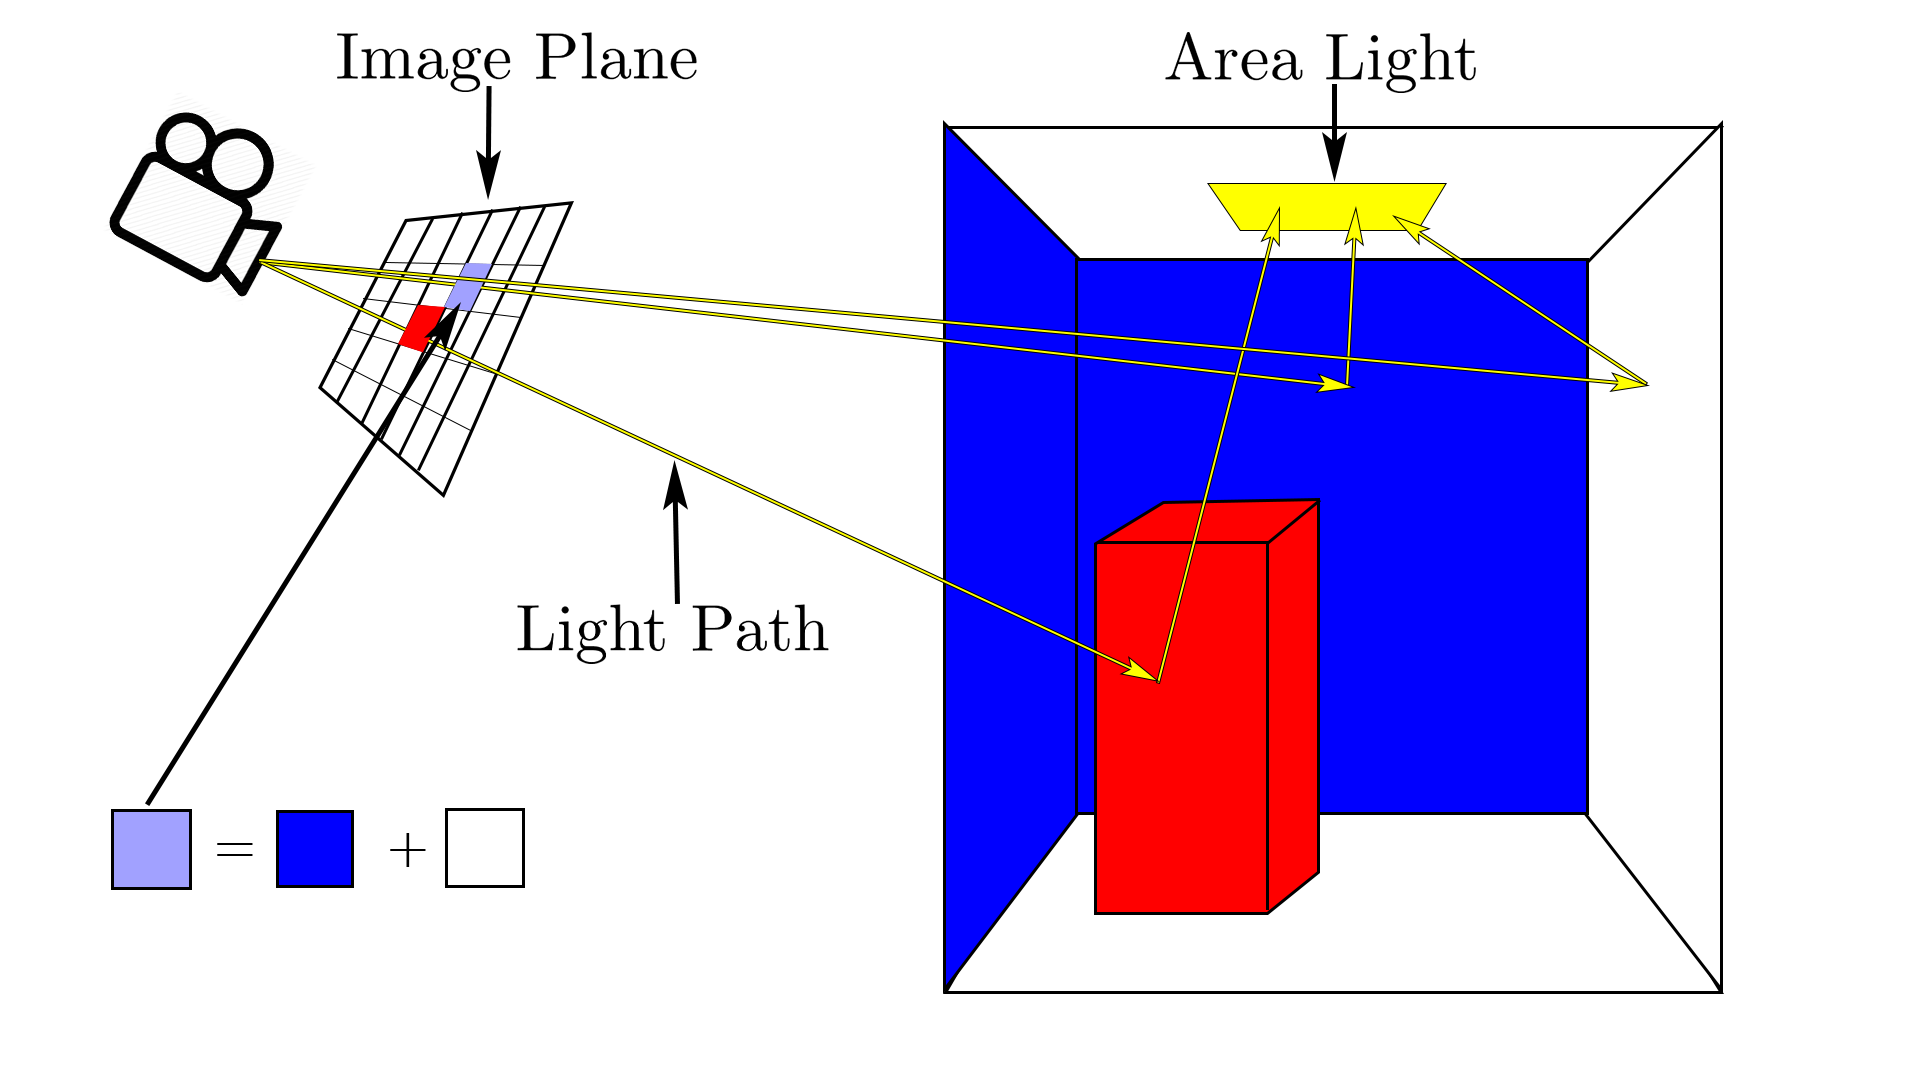
\includegraphics[width=0.8\textwidth]{images/path_tracing.png}    
\end{center}
\caption{An illustration of path tracing, where three light paths are traced from from the camera through a pixel, to the light source in a simple 3D scene.}
\label{fig:path_tracing_overview}
\end{figure}

Path tracing simulates global illumination, meaning it accounts for both direct and 
indirect illumination. Direct illumination being light paths emitted from a light 
source, which reflect off exactly one surface before reaching the camera in the 
scene . Whereas in indirect illumination, light paths reflect 2 or times before
reaching the camera. In Figure \ref{fig:direct_and_global}, an identical scene is shown with only direct illumination
(left) and the other with global illumination (right). The globally illuminated scene displays
a range of effects due to Path tracings ability to accurately simulate light transport, 
which is not the case for the directly illuminated scene. Where light transport simulation
refers to firing and summing up the contributions of light transport paths that connect from the
camera to light sources \cite{keller2016path}, such as those displayed in Figure \ref{fig:direct_and_global}. For 
example, effects such as; (a) colour bleeding which is clear on the white walls by the boxes. (b) Soft shadows of the boxes silhouette. (c) Indirect diffuse lighting
from light transport simulation causes the shadow of the box to not be pitch black.\\

\begin{figure}[h]
\centering
\begin{minipage}{.45\textwidth}
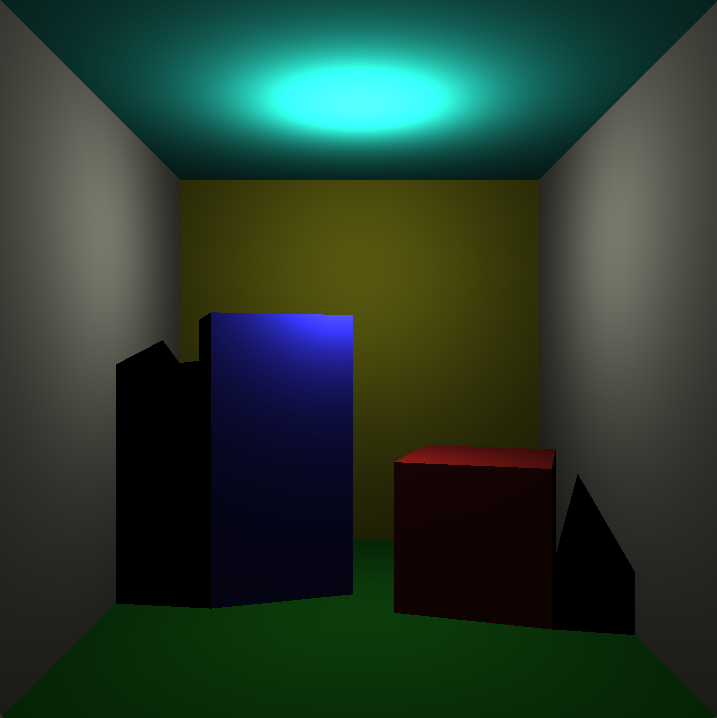
\includegraphics[width=0.99\textwidth]{images/renders/cornell/direct_light.png}    
\subcaption{Direct Illumination}
\end{minipage}\hspace{2em}
\begin{minipage}{.45\textwidth}
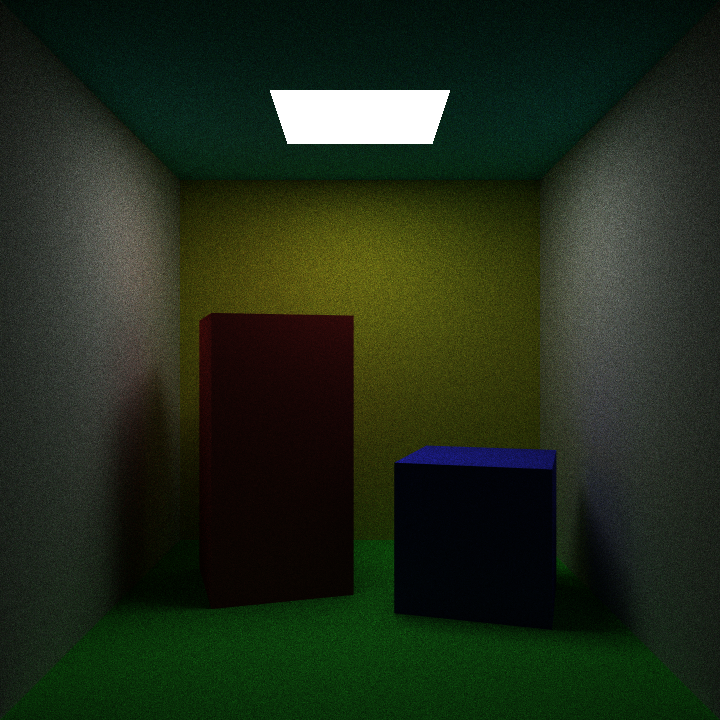
\includegraphics[width=0.99\textwidth]{images/renders/cornell/2048_300_default.png}    
\subcaption{Global Illumination}
\end{minipage}
\caption{Two renders of the Cornell Box, where the left is directly illuminated and the right is globally illuminated.}
\label{fig:direct_and_global}
\end{figure}

Light transport simulation methods are able to produce 
many complex light transport effects by a simple single pass of a rendering algorithm.
This allows artists to increase productivity and perform less manual image tweaking
in the production of photo-realistic images. Due to this, the Computer Graphics 
industry has seen a large resurgence in research and usage of light transport simulation 
rendering methods in the past decade \cite{krivanek2014recent}. \\

My work in this thesis focuses on developing and assessing importance sampling 
techniques using Temporal Difference learning methods for light transport simulation 
in forward Path tracing. In particular, More specifically,
for any intersection point in a 3D scene, I attempt to create an AI agent that learns 
and samples in  directions light is coming from, reducing the total number of 
zero contribution light paths. A zero contribution light path is one whose 
estimated colour values are almost zero for all $(R,G,B)$ components, hence,
they contribute almost no visible difference to the rendered image. We should 
instead focus our sampling on light paths which do contribute to the image,
reducing the noise in pixel values and bringing them closer to their true 
values for the same number of sampled rays per pixel. Meaning, Importance 
sampling can reduce the number of rays needed to be sampled per pixel in 
order to receive a photo-realistic (also known as converged) image from Path 
tracing. An example of this reduction in noise can be see in \ref{fig:noise_reduction_simple_room}, where the 
default forward path tracers output is compared to Nvidia's on-line
reinforcement learning Path tracer which uses Importance sampling. Note, any 
light transport simulation algorithm \cite{jensen1996global, keller2016path} can benefit from the Temporal DIfference learning
schemes which will be described, 
as they are all derived from what is known as the rendering equation. This equation
is used as a mathematical basis of modelling light transport.\\

\begin{figure}[h]
\centering
\begin{minipage}{.45\textwidth}
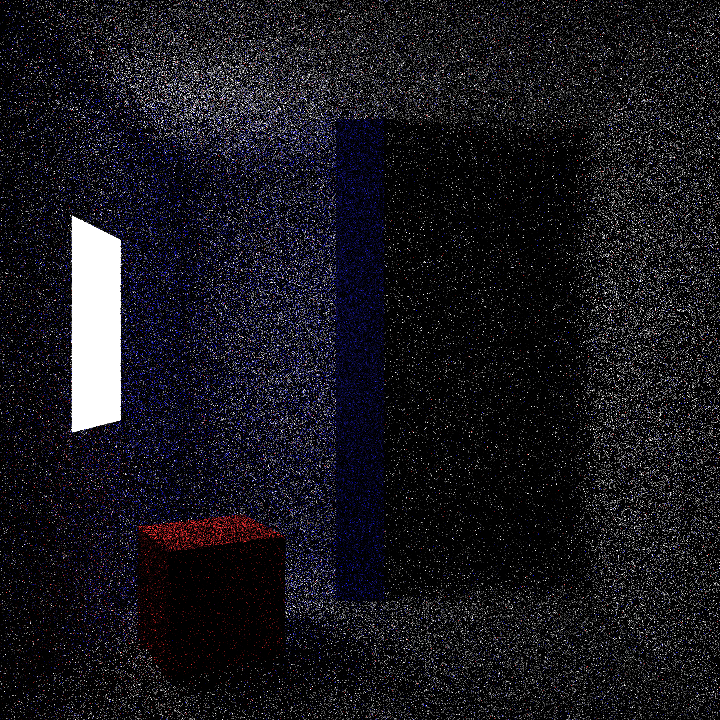
\includegraphics[width=0.99\textwidth]{images/renders/simple_room/default_16.png}    
\subcaption{Default Forward Path Tracer}
\end{minipage}\hspace{2em}
\begin{minipage}{.45\textwidth}
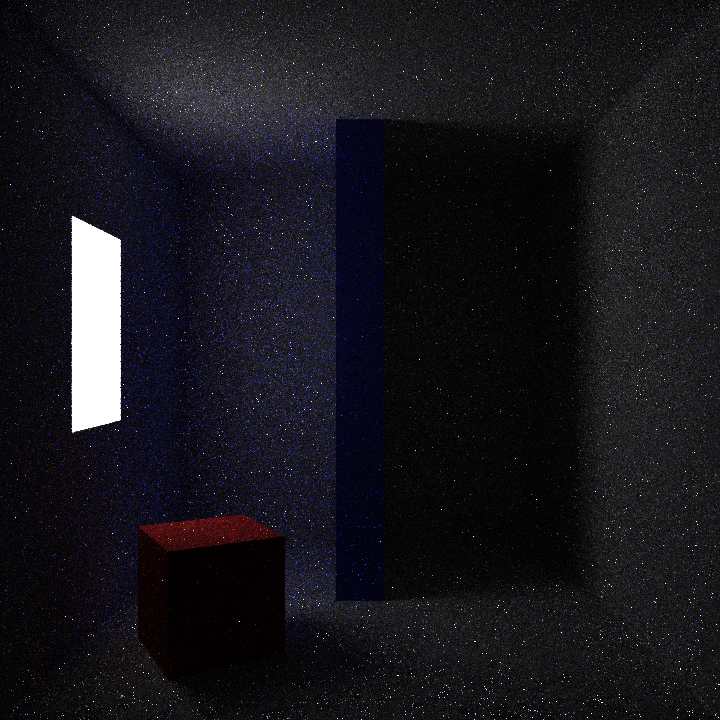
\includegraphics[width=0.99\textwidth]{images/renders/simple_room/reinforcement_16.png}    
\subcaption{Expected Sarsa Path Tracer}
\end{minipage}
\caption{Two renders of a simple room using 16 sampled light paths per pixel. Where one does not use importance sampling in the construction of light paths (left), and the other does so based on a reinforcement learning rule (right). A clear reduction in image noise can be seen.}
\label{fig:noise_reduction_simple_room}
\end{figure}

It is paramount that Importance sampling Path tracing algorithms continue to accurately
simulates global illumination in order to produce photo-realistic images in a single
rendering pass, as this is the major selling point of Path tracing over other 
methods. Therefore, I will also be assessing the accuracy of the global
illumination approximation made by the Importance sampling algorithms compared
to that of the naive forward Path tracing algorithm.

\section{Temporal Difference Learning for Importance Sampling Ray Directions}
\label{sec:td_learn_for_importance}

There are three important unanswered questions up to this point; a) what is temporal
difference learning?  b) How can temporal difference learning methods be 
used to importance sample new ray directions for a given intersection point in 
the scene? c) Why use temporal difference learning methods over other Importance 
sampling methods to do so? 

\subsection{What is Temporal Difference learning?}
Temporal difference learning, which I will refer to from 
here on as TD-learning, are a set of model free Reinforcement learning methods. 
Firstly, Reinforcement learning is the process of an AI agent learning what is the 
best action to take in any given state of the system it exists within, in order to 
maximise a numerical reward signal \cite{sutton2011reinforcement}.
The AI agent is not told which actions are  best to take in a given state, but
 instead it must learn which ones are by trialling them and observing the reward 
signal. Actions taken may not only affect the immediate 
reward, but all subsequent rewards received for taking future actions. For 
example, picture a robot rover whose duty it is to explore the surrounding area 
as much possible. A state in this case is a position in the world it is exploring, 
and its action are the directions to move in for a given distance. If it discovers 
a new area, it receives a positive reward signal. Now, if the robot chooses to 
explore a given area it may not be able to get back from, say a canyon, the 
robot is limited to searching areas reachable from the canyon. Hence, all 
subsequent reward signals are limited to what can be received from exploration 
of the canyon, compared to not entering the canyon and exploring areas which 
can be returned from first.

\begin{comment} %Might need to remove all
As mentioned TD learning methods are model free methods, meaning the methods 
do not require a model of the system dynamics they are placed in, instead they
 learn over time by interacting with the system. In other words, they learn from 
 raw experience  \cite{sutton2011reinforcement}. TD methods update their current
estimates based on a combination of data received from interacting with the 
environment, and partly on their current learned estimates without waiting for the 
final outcome of events, this is known as bootstrapping. To illustrate the concept 
of bootstrapping, imagine you are driving home from work and you wish to estimate 
how long it will take you get home. By following a TD learning method, if you hit 
traffic you can update your current estimate of the time it takes you to drive home
based on this new data, and your pre-existing estimate. Whereas compared to 
another set of Reinforcement learning methods known as Monte Carlo methods, 
you would have to wait until you got home to update your current estimate of how 
long it takes to get home from work. Meaning you have to wait for the final outcome
before learning can begin, which is not the case for TD learning.
\end{comment}

\subsection{Temporal Difference learning methods for Efficient Light Transport Simulation}

One of my main aims to reduce the number of zero contribution light paths sampled 
in Path tracing by the use of TD learning methods. In order to do so I must formulate 
the problem a reinforcement learning problem, which is done in detail in Chapter
\ref{chap:technical}. However for a conceptual overview it suffices to explain what a 
state, action, and reward signal will be in the case of light transport simulation within 
Path tracing:

\begin{itemize}

\item \textbf{State}: A 3D intersection position in the scene for a given ray to sample 
the rays next direction from. 

\item \textbf{Action}: Firing the ray in a given direction (3D vector) from the current 
state.

\item \textbf{Reward Signal}: The amount of light incident from the direction the ray 
was sampled in.

\end{itemize}

In this reinforcement learning setting, we can use TD-learning methods to create 
an AI agent which learns by taking different actions in different states and observes 
their reward signals to find out for each state which actions have the highest valuations.
By then converting the action space into a probability distribution weighted by each
actions learned valuation, the AI agent will more likely sample non-zero contribution 
light paths, reducing noise in rendered images. Note, the term valuation means the 
total expected reward for taking a given action, meaning valuation not only accounts 
for the immediate reward, but the expected reward for taking all future actions to come 
until the ray intersects with a light. Also, for the proposed AI agent, current actions 
can affect future rewards, as when the ray intersects a surface it looses some energy. 
Therefore, future rewards received after many intersections will be discounted 
compared to the reward of received immediately to match this behaviour. This means 
the agent will aim to minimise the average number of intersection a ray makes before 
intersecting with a light source, making it a good metric to test evaluate against to 
determine how well the AI agent is performing.

\subsection{Why use Temporal Difference Learning for Importance Sampling?}

Traditional Importance sampling techniques for path tracing do not take into account 
the visibility of the object from light source. A light blocker is shown in \ref{fig:blocker}, where the 
blocking object stops rays from directly reaching the light. Due to the unknown 
presence of blockers, traditional importance sampling methods can fail to avoid 
sampling zero contribution light paths. Therefore, scenes which are significantly 
affected by blockers will not receive the benefits from traditional Importance sampling 
and can even benefit more from an uniform sampling scheme 
\cite{ramamoorthi2012theory}.\\

\begin{figure}[h!]
\begin{center}
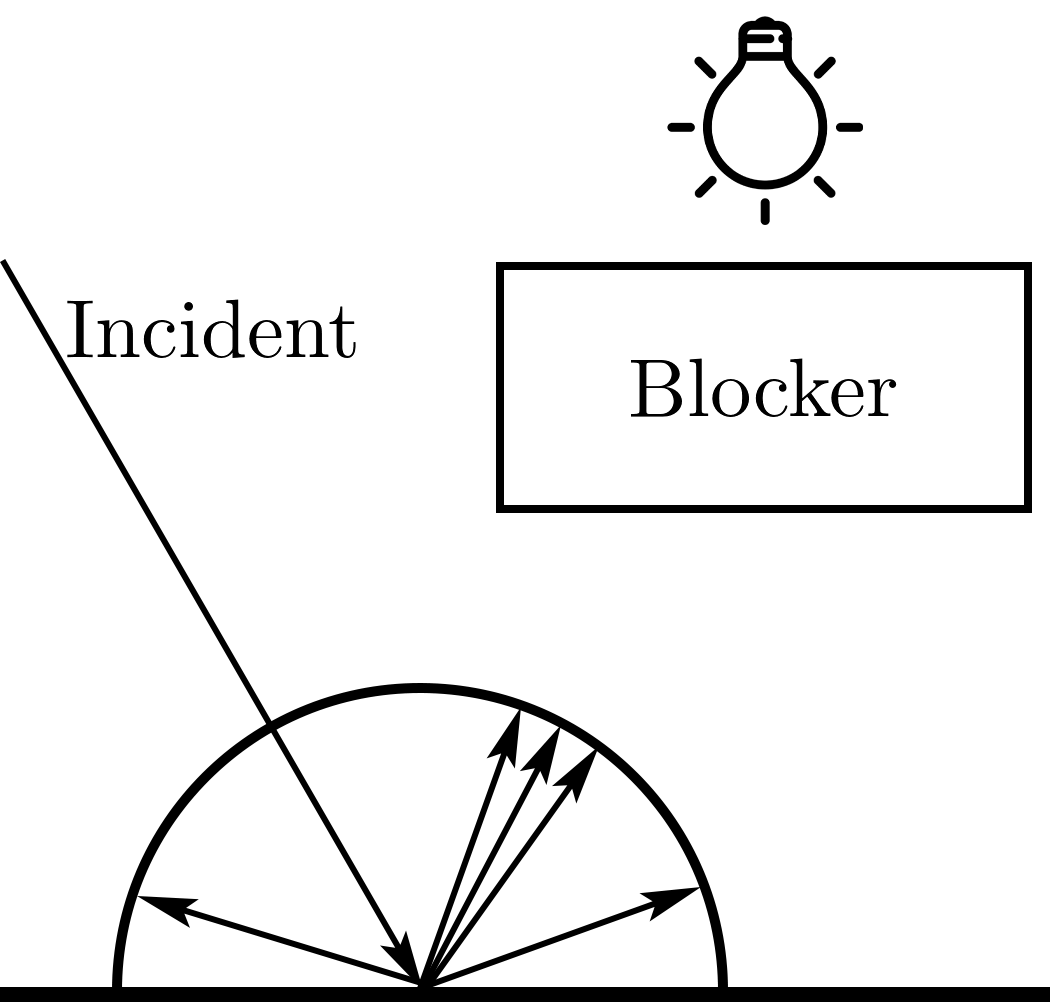
\includegraphics[width=0.3\textwidth]{images/light_blocker.png}    
\end{center}
\caption{An illustration of a light blocker for an importance sampling scheme which does not consider visibility. Each arrow represents a possible direction the light path will be reflected in. Clearly the reflected light path is likely to hit the blocker increasing the likelihood of it becoming a zero-contribution light path.}
\label{fig:blocker}
\end{figure}

Temporal difference learning methods are better equipped to tackle this problem 
\cite{dahm2017learning}. As the AI agent described in the previous section learns 
which directions light is coming from in the scene and concentrates its sampling 
towards these directions. Directions leading to blockers will have a low value, 
hence it is unlikely the AI agent will sample rays in these directions.\\

\section{Motivation}
\label{sec:motivation}

Rendering time of my graphics engine is not something I have tried to heavily 
optimise. I instead focus on producing higher quality images using the same 
number of samples per pixel in light transport simulation in hope that future 
work will find ways of optimising my methods for speed. Therefore, my work 
still aims to contribute to the wider goal seen in computer graphics to use 
accurate light transport simulation in the rendering of photo-realistic images 
for complex scenes in real-time.  Speeding up the methods I use is a large 
topic in itself, requiring a deep investigation into the best software, hardware, 
and parallel programming paradigms to use.\\

\subsection{Real time Rendering using Accurate Light Transport Simulation}
The motivation for using accurate light transport simulation in real-time 
comes from the clear superior visual quality of images rendered using this 
techniques, compared to that of scanline methods which are currently used. 
Where scanline rendering, also known as rasterizing, is the current computer 
graphics industry standard method for real-time rendering. Not only are 
renders for a wide range of scenes clearly superior from methods which 
accurately simulate light transport, but they also scale far better with the 
number of polygons used to build the scenes surfaces. Therefore, scanline 
rendering for scenes with extremely complex geometry in real-time is currently 
not and option. Accurate light transport simulation methods therefore have 
great potential to be used in ultra realistic simulations for applications such 
as scenario planning and virtual reality learning environments \cite{pan2006virtual}. 
Also, many games sell realism as one of their most important features, therefore 
developing photo-realistic graphics in real-time has clear economic incentive for 
the video games industry which was valued at over \$$136$ by the end of 2018 
\cite{bloomberg.com}. An economic incentive can also be seen for the film
industry, where reductions in render times lead to a direct saving on compute 
time, as well as the hardware required to render full length films.

\subsection{Recent Developments}
Due to the incentives, a large amount of research and investment has been focused 
on purpose built hardware and Deep learning  post-processing methods in an 
attempt to bring accurate light transport simulation into real-time. NVIDIA's 
Turing Ray Tracing Technology \cite{nvidia_turing_architecture_whitepaper_2018} 
represents a significant leap in the hardware to support light transport simulation. 
It allows for real-time graphics engines to be a hybrid of both scanline rendering, 
and ray-tracing. The 20 series Turing GPU architecture has significantly improved 
the speed of ray-casting for light transport simulation, and has the capacity for  
simulating 10 Giga Rays per second. However, using this hardware alone with 
current rendering methods is not enough to perform accurate light transport 
simulation for complex scenes in real-time.\\

Post-processing methods are designed to take a noisy input image produced by a 
render which simulates light transport, and then reconstruct the image to remove 
the noise present in the image. Generally these methods rely on pre-trained deep 
neural networks to reconstruct the image far quicker then it would take for the 
renderer to produce an image of the same visual quality \cite{bako2017kernel}. 
Once again NVIDIA has made significant advancements in this area with NVIDIA 
OptiX AI Accelerated Denoiser, which is based on their newly designed recurrent 
denoising autoencoder \cite{chaitanya2017interactive}. OptiX has been successfully 
integrated in to many of the top rendering engines which accurately simulate light
transport, such as RenderMan \cite{christensen2018renderman} and Arnold 
\cite{georgiev2018arnold}. Whilst post-processing has significantly reduced the 
number of samples required to render photo-realistic images, there is still more 
work to be done to produce these images in real-time.\\

By using importance sampling by TD learning to reduce the number of samples 
required for accurate light transport simulation, the same standard of noisy 
image can be fed into an AI accelerated denoiser with fewer samples per pixel 
in light transport simulation. Running a rendering engine optimised in this way on 
purpose built hardware could make accurate light transport simulation for 
rendering photo-realistic images closer than it ever has been to real-time.

\section{Challenges and Objectives}

% Needs work

As previously mentioned, there already exists an example of TD learning used 
for importance sampling ray directions in a forward Path tracer \cite{dahm2017learning}. 
However, further methods of analysis need to be conducted upon this new 
method to determine its performance for reducing the number of zero contribution l
ight paths for different scenes with different settings. It is difficult to assess this as 
there are infinitely many scenes the method can be used to render, so coming to a 
clear conclusion is difficult. Another difficult task is that of designing an algorithm 
for an AI agent to learn what are the favourable directions to sample in a scene are 
using the deep Q-learning method. This includes some important unanswered 
questions, such as; is it possible for a deep neural network to model all Q values for 
a continuous scene space? If so, what is a suitable network architecture? All of 
which I will describe in more depth in Chapter \ref{chap:deep-q}. Then the actual 
task of implementing such an algorithm in a graphics engine written from scratch 
is non-trivial due to the technologies which will need to be combined together. 
The algorithm must also run fast enough to collect large amounts of data from, 
otherwise a justified conclusion on its performance cannot be made. Therefore, 
the algorithm will have to be parallelized and run on a GPU.\\

As previously mentioned, my main goal is to investigate the ability of two 
different temporal difference learning algorithms ability to reduce the number 
of zero contribution light paths in path tracing, whilst still accurately 
approximating global illumination. Which can be broken down in to the 
following objectives:

\begin{enumerate}
\item Reimplement Nvidia's state of the art on-line Temporal 
Difference learning Path Tracer in order to further investigate its ability
to reduce the number of zero contribution light paths.

\item Design and implement an on-line Deep Q-Learning variant of the
Path tracing algorithm and investigate its ability to reduce the number of zero contribution light paths sampled.

\item Assess both Nvidia's state of the art on-line Temporal Difference 
learning Path tracer, and the Deep Q-Learning Path tracer' on their ability 
to accurately simulate Global Illumination.

\end{enumerate}


\begin{comment}
{\bf A compulsory chapter,     of roughly $5$ pages}
\vspace{1cm} 

\noindent
This chapter should describe the project context, and motivate each of
the proposed aims and objectives.  Ideally, it is written at a fairly 
high-level, and easily understood by a reader who is technically 
competent but not an expert in the topic itself.

In short, the goal is to answer three questions for the reader.  First, 
what is the project topic, or problem being investigated?  Second, why 
is the topic important, or rather why should the reader care about it?  
For example, why there is a need for this project (e.g., lack of similar 
software or deficiency in existing software), who will benefit from the 
project and in what way (e.g., end-users, or software developers) what 
work does the project build on and why is the selected approach either
important and/or interesting (e.g., fills a gap in literature, applies
results from another field to a new problem).  Finally, what are the 
central challenges involved and why are they significant? 
 
The chapter should conclude with a concise bullet point list that 
summarises the aims and objectives.  For example:

\begin{quote}
\noindent
The high-level objective of this project is to reduce the performance 
gap between hardware and software implementations of modular arithmetic.  
More specifically, the concrete aims are:

\begin{enumerate}
\item Research and survey literature on public-key cryptography and
      identify the state of the art in exponentiation algorithms.
\item Improve the state of the art algorithm so that it can be used
      in an effective and flexible way on constrained devices.
\item Implement a framework for describing exponentiation algorithms
      and populate it with suitable examples from the literature on 
      an ARM7 platform.
\item Use the framework to perform a study of algorithm performance
      in terms of time and space, and show the proposed improvements
      are worthwhile.
\end{enumerate}
\end{quote}


\textbf{Preliminary}
\begin{enumerate}
\item Path-tracing in industry/ray-tracing in general, why is it important 
and how is the current field moving. Why should we optimise it algorithmically. 
Why should the reader care about path-tracing? - Usage in films, increasing
 interest for real-time simulations and gaming industry which is worth lots of money

\item High level overview of path-tracing: specifically must explain why it takes 
so long and why we care about the number of samples

\item In the path-tracing algorithm, a single pixel's colour is determined by firing 
multiple rays from the camera, through that pixel into the scene and building a 
colour value estimate for each one, then averaging their values to get the pixels 
colour. Each rays colour estimate is computed by estimating a solution to the recursive
Rendering Equation (cite). The path-tracing algorithms estimate to this solution involves 
scattering the ray around the scene until it intersects with a light source. Therefore, if a
 ray is scattered in a direction with zero-light contribution, but other sampled rays are not,
  a noisy estimate is achieved for the pixel value unless many rays are sampled to 
  reduce the effect of this noise. Therefore, avoiding  scattering rays in directions of 
  zero-light power contribution can reduce the number of samples needed to achieve 
  an accurate estimate of a pixels colour value.

\item Work was primarily motivated by Ken \& Dahms paper for modelling the irradiance
 distribution in order to reduce the number of zero-contribution light transport paths 
 traced. Nvidia are world leaders in GPU manufacturing and drive the computer 
 graphics forward.

\item Literature around efficiently simulating light transport - it's applicability to all 
modern used off-line rendering techniques

\item Aims \& Challenges:

\begin{enumerate}
\item Implementing a path-tracer for diffuse surfaces from scratch using only maths 
and pixel libraries as helper functions which can handle imports of a custom scene
\item Accelerating path-tracer on Cuda to get results in a reasonable time
\item Implementing the irradiance volume data-structure and sampling technique which 
can adapt to any size scene
\item Implementing Ken Dahms proposed path-tracing algorithm with nearest neighbour
 search of KD-Tree on a GPU efficiently 
\item Researching reinforcement learning: TD-Learning \& deep reinforcement learning - 
never been taught before, so self taught with resources on-line
\item Training a network on pre-computed Q values to check if it is possible for a neural
 network to learn the irradiance distribution function for a set of points in a scene
\item Designing an algorithm to integrate deep reinforcement learning into the 
rendering pipeline for a path-tracer
\item Choosing a set of metrics to evaluate the algorithms performances on
\item Accelerating the algorithms via Cuda to run on Nvidia GPU
\end{enumerate}

\end{enumerate}
\end{comment}

\end{document}